\section{Implementation of Dynamic Honeycomb Maze}

The design of this maze has three basic interacting units.
They are:
\begin{enumerate}
    \item The \textbf{\textit{Animal}}, which makes a decision about which platform it would like to move to.
    \item The \textbf{\textit{Robot}s}, which  move around grid as required to give the animal the choices about where it would like to move to next.
    \item The \textbf{\textit{Maze}}, which is the set of all points in the grid within which the robots can navigate around in.
\end{enumerate}
As such the program has been structured into these three basic parts where the relevant functions are placed into the relevant classes.

\subsubsection{\textit{Inner Ring}, \textit{Outer Ring} and \textit{Relative Position}}

% The idea the platforms have to compute their distance in correlation to each other, not based on their absolute distance in the maze from each other

% Because of how often these ideas are used in the code, the inner ring, outer ring and relative position are used introduced at the start of the program

% Because of the importance of these two ideas in the development of this algorithm these two ideas have been introduced before the explanation of where they are used in the algorithm.

The movement of the robots occur in relation to each-other, for example 'a movement \textit{away} from another robot' or '\textit{around} each other'. As such  these relative heuristics are developed for computing the robots' place in relation to each-other and are used in many parts of the program to compute moves.

\paragraph{Inner and Outer Ring}

The \textit{inner ring} is the set of 6 hexagonal tiles that are consecutive to one central tile. These are the orange tiles in Fig \ref{fig:inner_ring}.
The \textit{outer ring} are the set of 12 tiles that are all exactly 2 moves away from the central tile (blue tiles in Fig \ref{fig:inner_ring})
Often the inner and outer ring will be computed from the animal robot position (as shown in Fig \ref{fig:inner_ring}). See function \ref{function:def_inner_ring} for implementation.

\paragraph{Relative position}

Relative position acts as a mapping of all the six hexagonal points on the inner ring to point on the outer ring where relative position is defined. This come in useful when setting path-finding targets in Section \ref{section:pathfinding_targets}.
See function \ref{function:def_relative_position} for implementation. t


\begin{figure}[H]
    \centering
    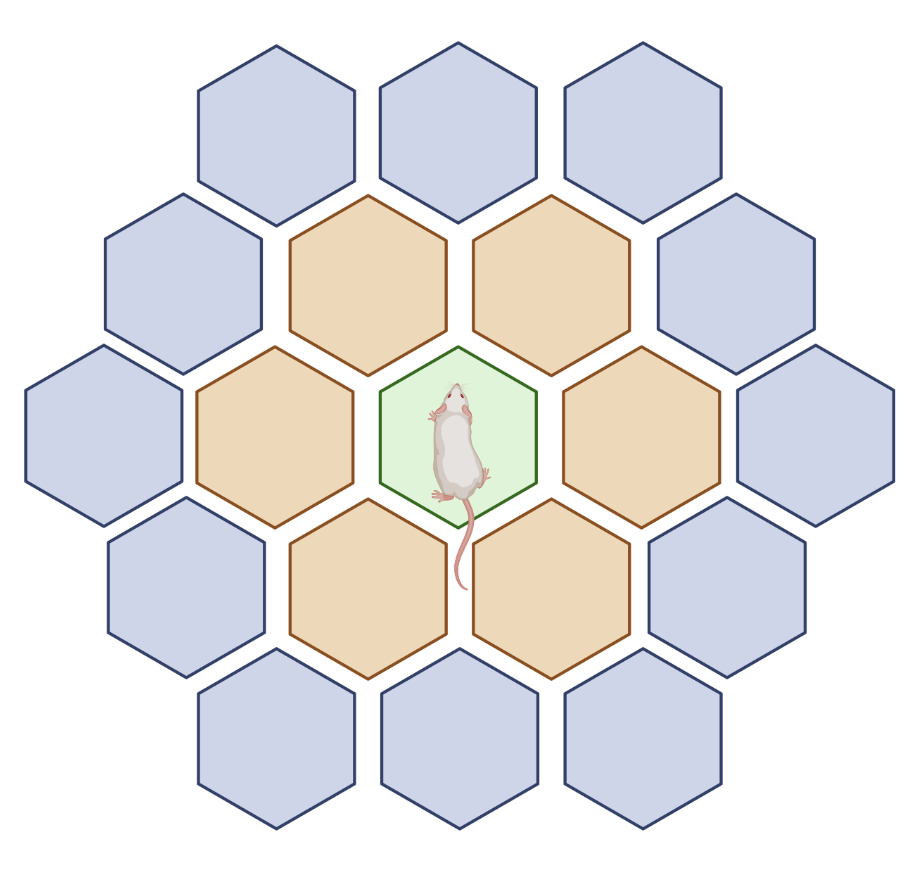
\includegraphics[scale = 0.5 ]{images/outer_rings.png}
    % 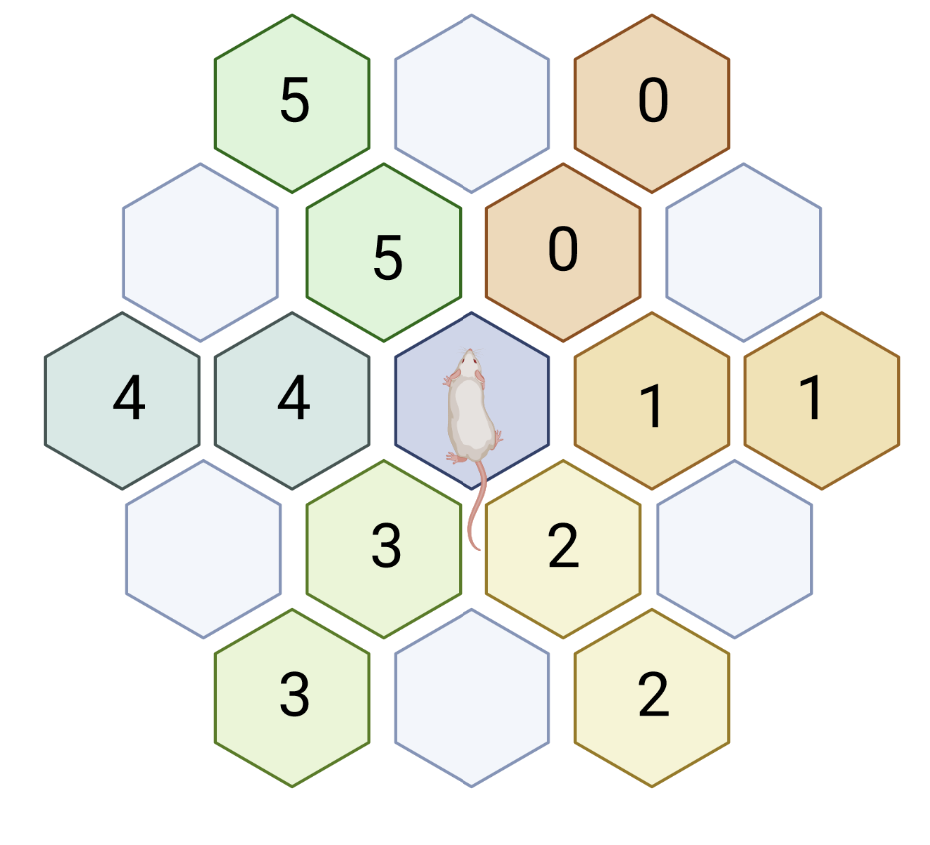
\includegraphics[scale = 0.50]{images/relative_position.png}
    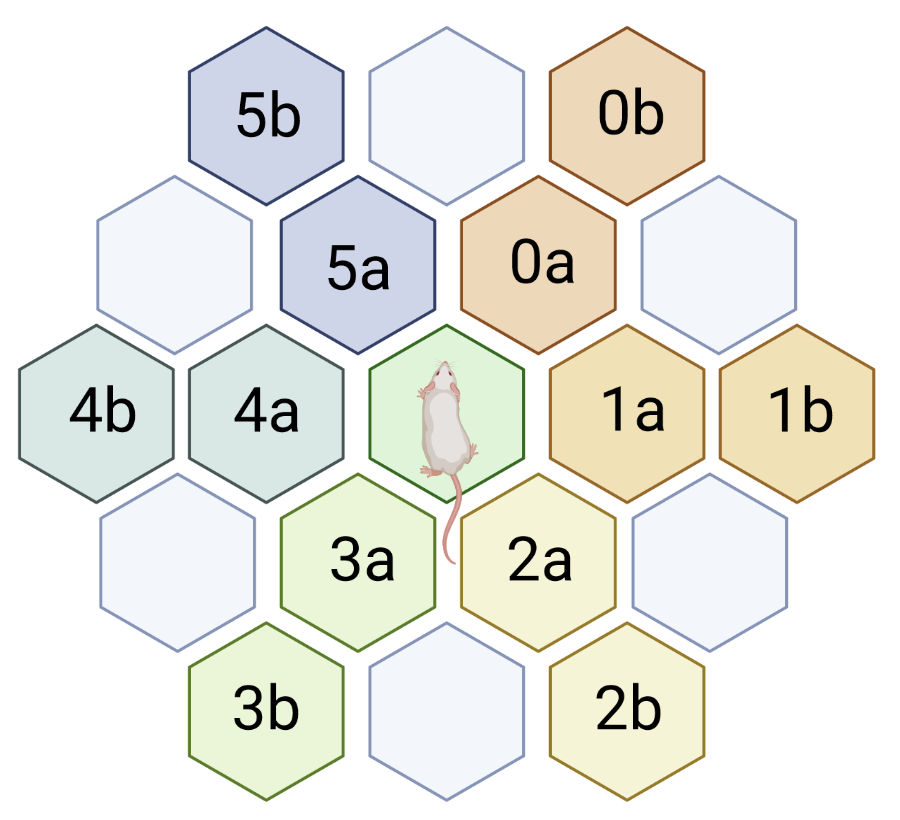
\includegraphics[scale = 0.50]{images/relative_position_mapped.png}
    \caption{This figure shows two important concepts that have been developed: 1. LHS: Inner (\textit{Orange}) and Outer Ring (\textit{Dark Blue}). 2. RHS: Relative Position}
    \label{fig:inner_ring}
\end{figure}


\subsection{\textit{Maze} Class}


This is the class which handles the area which the robot platforms move around.
It is important, for handling the boundaries of the maze, defining where robots are allowed to move without letting the path finding algorithm running out of space to complete its moves.

\subsubsection{Coordinate system}

Despite the surface on which the platform move around on being a 2D space, for the task as hand it is can be more intuitive to use a 3D coordinate system to encode the space traversed by the robots. This is because there are six directions the platforms can move out of any point in the grid. This can be thought of as three dimensions (where there is a backwards and forwards direction for each of the three dimensions). These are: the $North-East$ direction, the $East-West$ direction and the $North-West$ direction.
For this program, it has been decided that movement in the $North-East$ direction has been considered to be the positive $y$ direction, $East-West$ direction to be the positive $z$ direction and the $North-West$ direction to be considered positive $x$ direction and vis versa.

The mathematical embedding of this space is a slice through 3D coordinate system, taken through a diagonal of a cube and what is left is a hexagonal shape (exemplified by Fig. \ref{fig:hexagona_slice_through_cube}), more specifically the plane:
$$x + y + z = 0$$
 
This forms a hexagonally tiled surface can be used to as the plane on which out robots move through.

Based on theses rules the following figure shows the coordinate space that has been used. 
\begin{figure}[h]
    \centering
    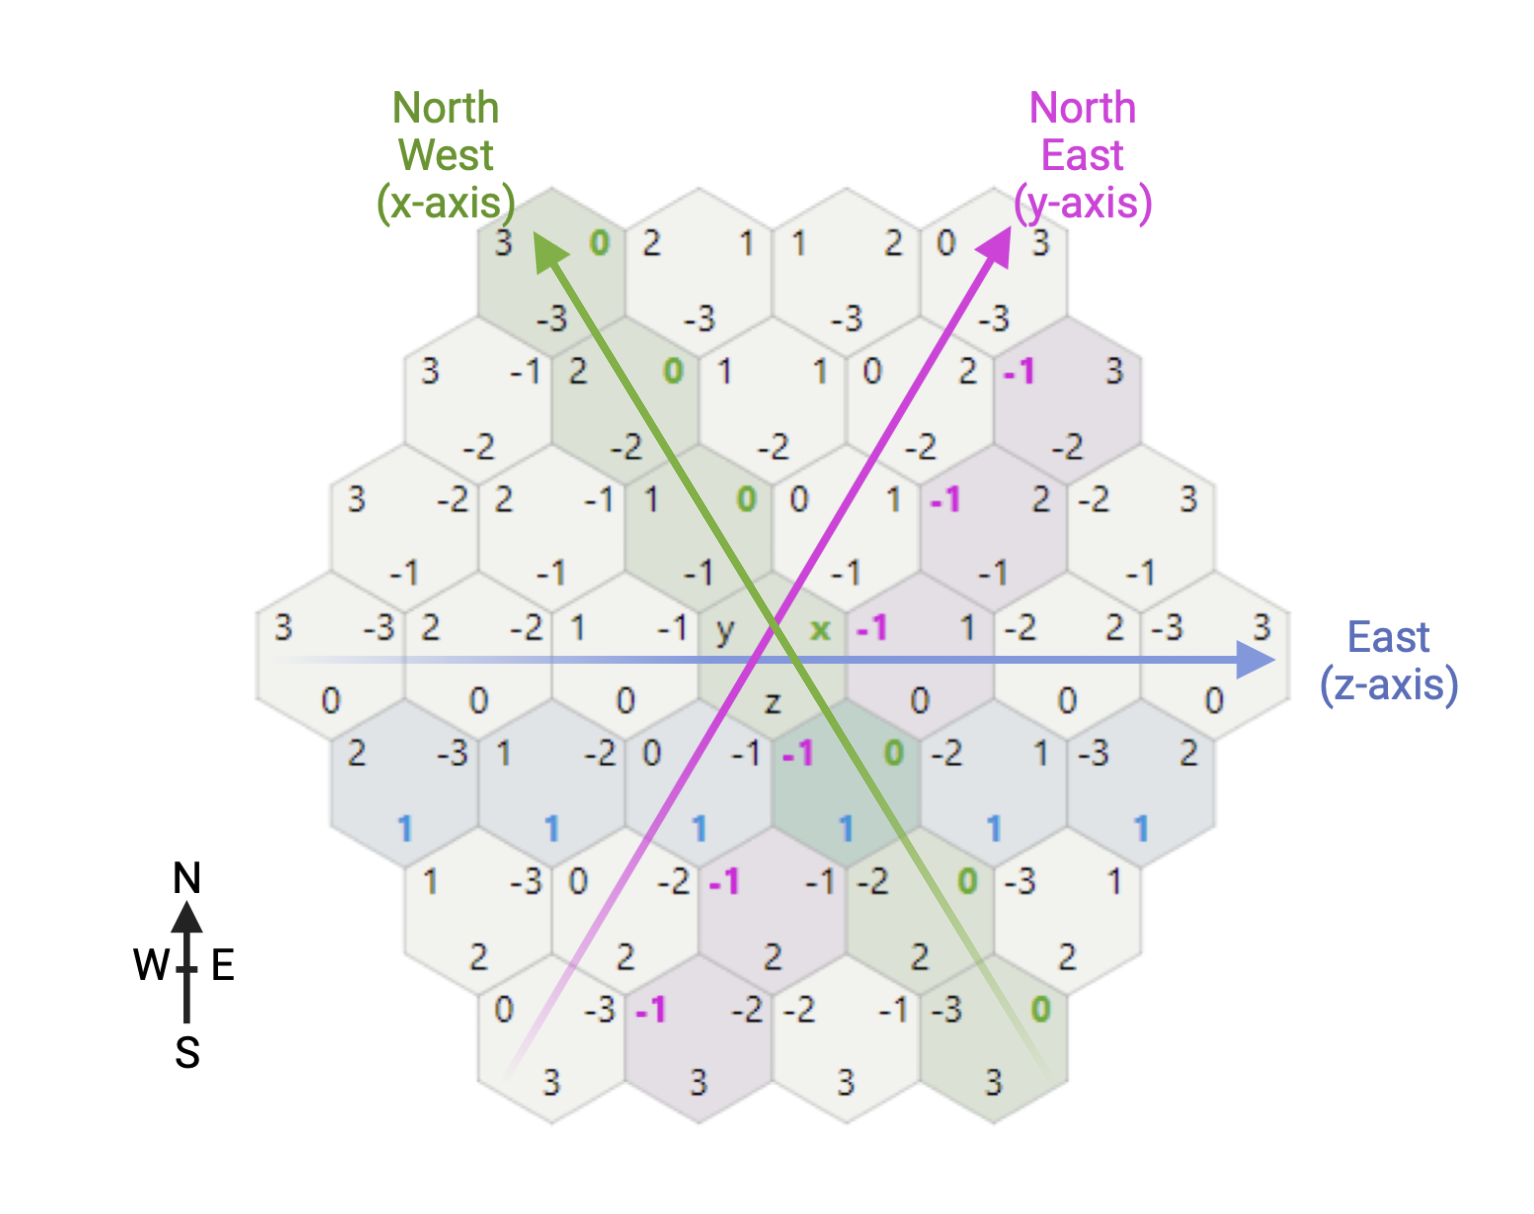
\includegraphics[scale=0.35]{images/hexagon_coordinates_adapted.png}
    \caption{The coordinate system used to encode the 2 dimensional space with a 3D coordinate system. The axis have been defined $North-West$ as $x$, $North-East$ as  $y$ and $East-West$ as $z$. This figure has been adapted from Red Blob Games \cite{patel_2021}}.
    \label{Hexagonal grid coordinates}
\end{figure}

Due to the novel coordinate system being used, a function has been defined in the \textit{Robot Class} which moves the robot around the coordinate space in a way that ensures the robots position remains valid (see Function \ref{function:move_around_hex_grid}).

\pagebreak
\subsection{\textit{Robot} Class}

This is the class which deals with the movement of the robot around the maze in which it is places. Notably, this includes the path-finding algorithm for the robots to move from the initial position to their final position and all the supporting functions required.

\subsubsection{Overview of the whole path-finding process}

The order of the overall algorithm requires the following steps:
\begin{tcolorbox}
\begin{enumerate}
    \item Deciding the order by which the platforms move so that no collisions take place. (See  Section \ref{section:order_of_operations})
    \item Movement of the platforms away from the animal robot so it can move freely without collision. (See Section \ref{section:pre_pathfinding})
    \item Path-finding around the board to their path-finding targets using the Dijsktra Path-finding Algorithm. (See Section \ref{section:pathfinding})
    \item Moving into the inner ring of the animal robot so they are in the new positions so that they are consecutive to the animal allowing the animal can make another decision to choose another platform around the maze. (See Section \ref{section:post_path_finding})
\end{enumerate}
\end{tcolorbox}


\begin{figure}[h]
    \centering
    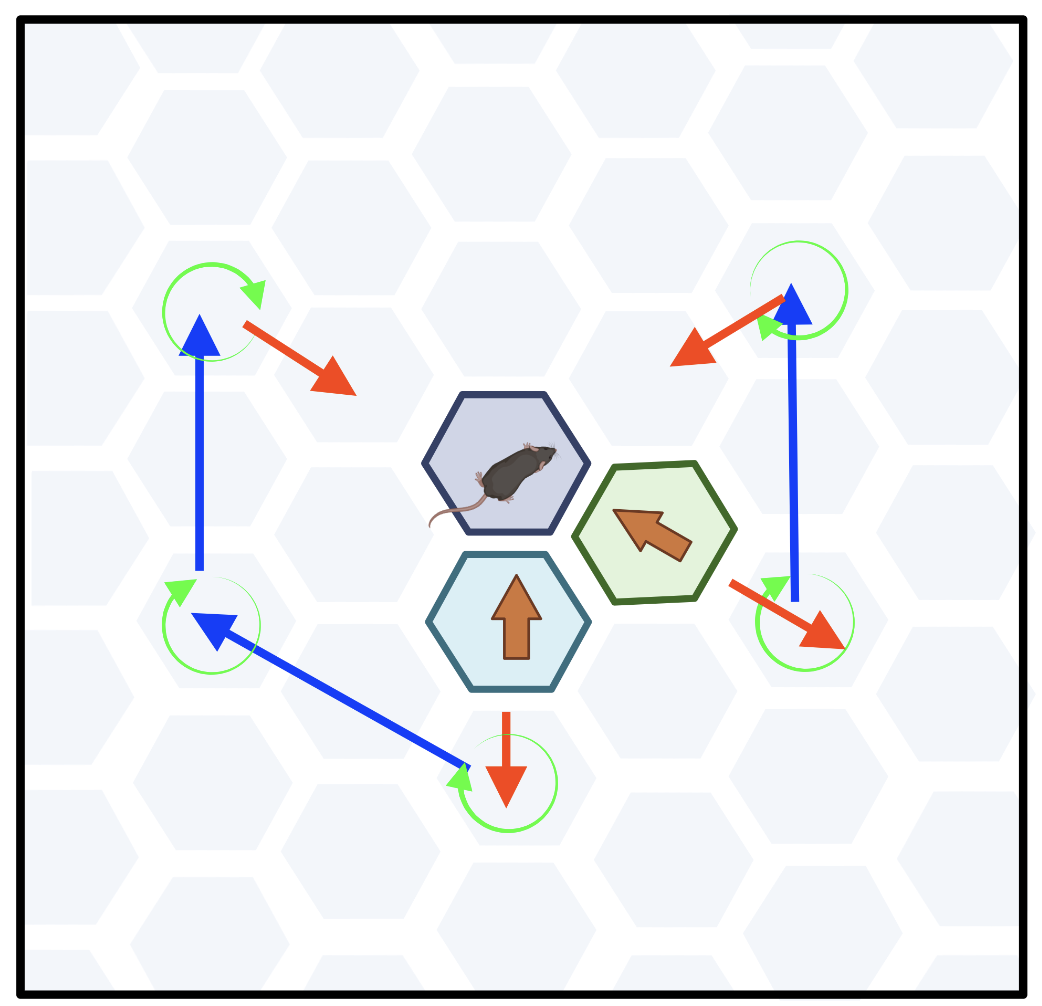
\includegraphics[scale=0.4]{images/overview_of_algorithm.png}
    \caption{This shows an example of the overall movement that would occur when moving the robot around}
    \label{fig:overview_of_algorithm}
\end{figure}

\subsubsection{Order of movement of the platforms}
\label{section:order_of_operations}
Here we discuss the order of operations for that the two moving platforms must take as to not collide with each other. There must be no collisions for all possible pairs of positions of the non animal robots around the animal robot.

From Fig \ref{fig:post_decision_states} (and panel C from Fig \ref{fig:control_flow_diagram}) we see that the platform which the animal did not choose to move on to, must be the first platform to move backwards away from the robot which used to have the animal on it. If this occurs, the platform is never consecutive to the other two platforms meaning it has free range of movement to start the path-finding phase.

After this has occured, the robot animal on it and the robot which used to have the animal on it left consecutive to each other (so there is limited range of movement).

The robot, with no animal on it, that is left consecutive to the (current) animal robot must always step back into the outer ring of the (current) animal robot. Similarly, this allows the robot free range of movement as it is not consecutive to any other robots.

These two observations imply: (1) that the robot not selected must always move first, and (2) the robot that used to be the animal robot must always move second.

It follows from this that the concept of 'animal robot', 'non-animal robot' and 'non-non-animal robot' can be developed.
\begin{tcolorbox}
They are defined in the following way:
\begin{itemize}
    \item \textbf{'Animal Robot' (AR)} is the platform robot that the animal has choose to move to. This will always be \textbf{stationary} during the path-finding method.
    \item \textbf{'Non-animal Robot'(NAR)} is the platform robot that the animal has come from. This will always be the \textbf{second} robot to move in the path-finding method.
    \item \textbf{'Non-non-animal robot' (NNAR)} is the platform robot that the animal has not chose from the two choices. This will always be the \textbf{first} robot to move for the path-finding method.
\end{itemize}
\begin{center}
\textit{From now, the above notation will be used}
\end{center}
\end{tcolorbox}



Associated with this is the table for reassigning the robots' state, based on their previous state and new state which is shows in Table \ref{table:change_states_of_robot}).

Using this framework for choosing the order in which the moves must take place, it can be shown that the NNAR must always move first to prevent the colliding of platform robots as they are consecutive. 
This prevents there ever being arrangements of robots where the order of operations has to be calculated due to the arrangement of the direction of the robots.

\subsubsection{Pre-Pathfinding Phase}
\label{section:pre_pathfinding}

Recall: the animal will be given a decision about which platform to move to. Once this has occurred, the maze will be left with the configurations shown in Figure \ref{fig:post_decision_states} and appendix Figure  \ref{fig:all_post_decision_states}.



\begin{figure}[h]
    \centering
    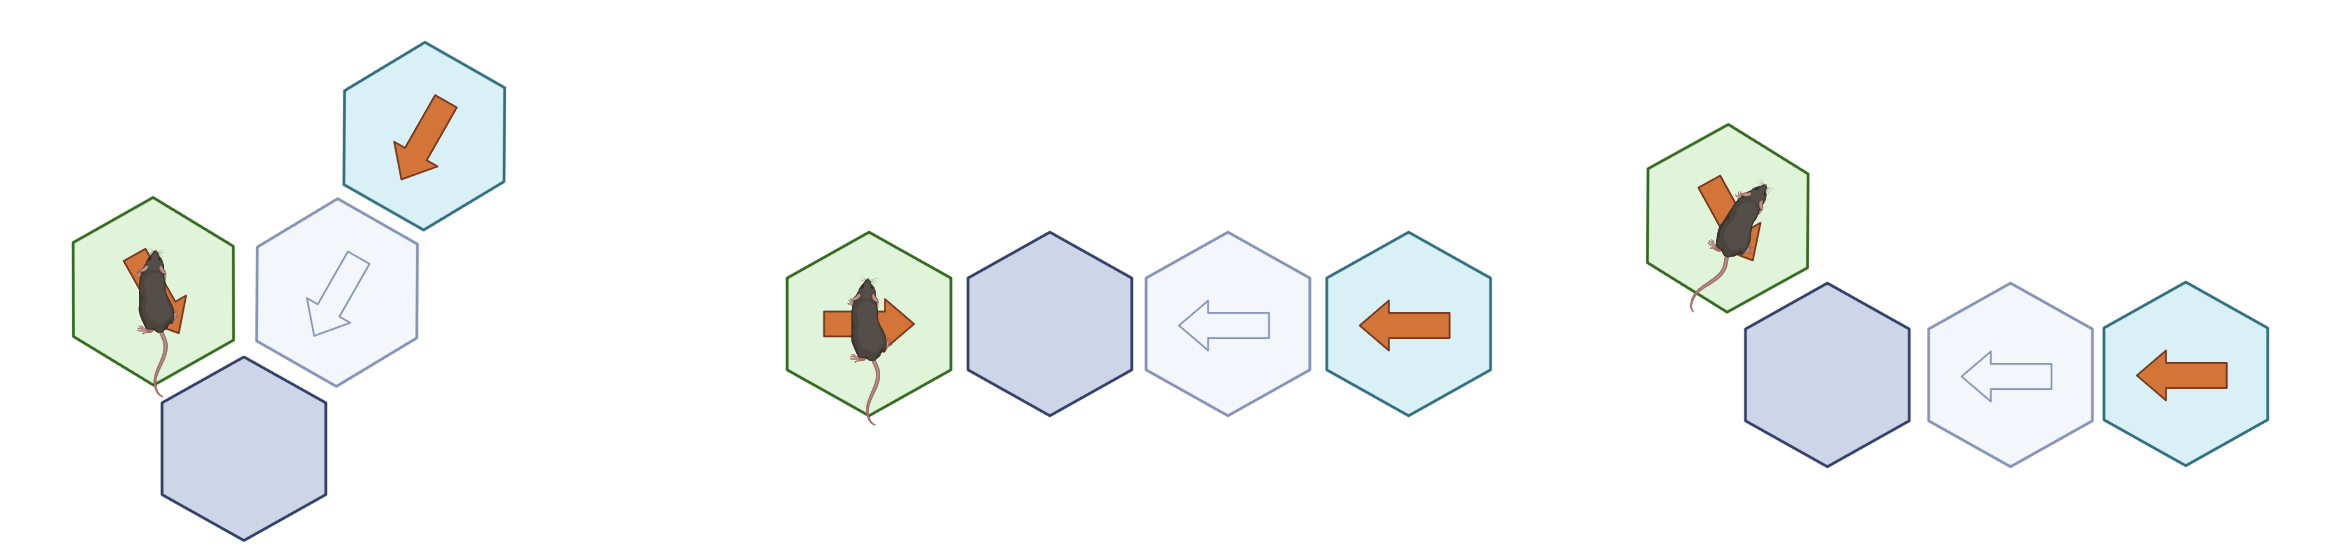
\includegraphics[scale = 0.5]{images/post_decision_state.png}
    \caption{This shows all possible arrangements of the three robots just after the animal has made a decision about which platform to stand on. In this case, the animal started on the blue platform as chose the green platform to stand on afterwards. \\ This demonstrates that the 'non-non-animal robot' must always step one step backwards from the other two robots to makes sure there are no other robots that are consecutive to it before it starts pathfinded to the outer ring position of the relative position of the path-finding end point.\\ \textbf{Note:} The \textit{dark blue} hexagon is the \textit{Non-animal robot (NAR)}, the \textit{green} hexagon is the \textit{Animal Robot (AR)} and the outlined hexagon is the \textit{Non-non-animal Robot (NNAR)}}
    \label{fig:post_decision_states}
\end{figure}

The strategies that are required for the \textit{Non-animal robot} and the \textit{Non-non Animal robot} are different and hence are handled differently. 

\paragraph{Non-non Animal Robot (NNAR)}

As demonstrated in Fig. \ref{fig:post_decision_states}, the NNAR must always move backwards away from the NAR. This is because this move will ensure that the NNAR is always not consecutive to any of the other robots in the system and hence free to move around.

\paragraph{Non-Animal Robot (NAR)}

Demonstrated in Panel D and E in Fig \ref{fig:control_flow_diagram}, the NAR must always move to the outer ring of AR, without turning. (Note: that this is sometime a step backwards and sometime a step forwards, depending on the rotation of the AR at the time.)

\begin{figure}[h]
    \centering
    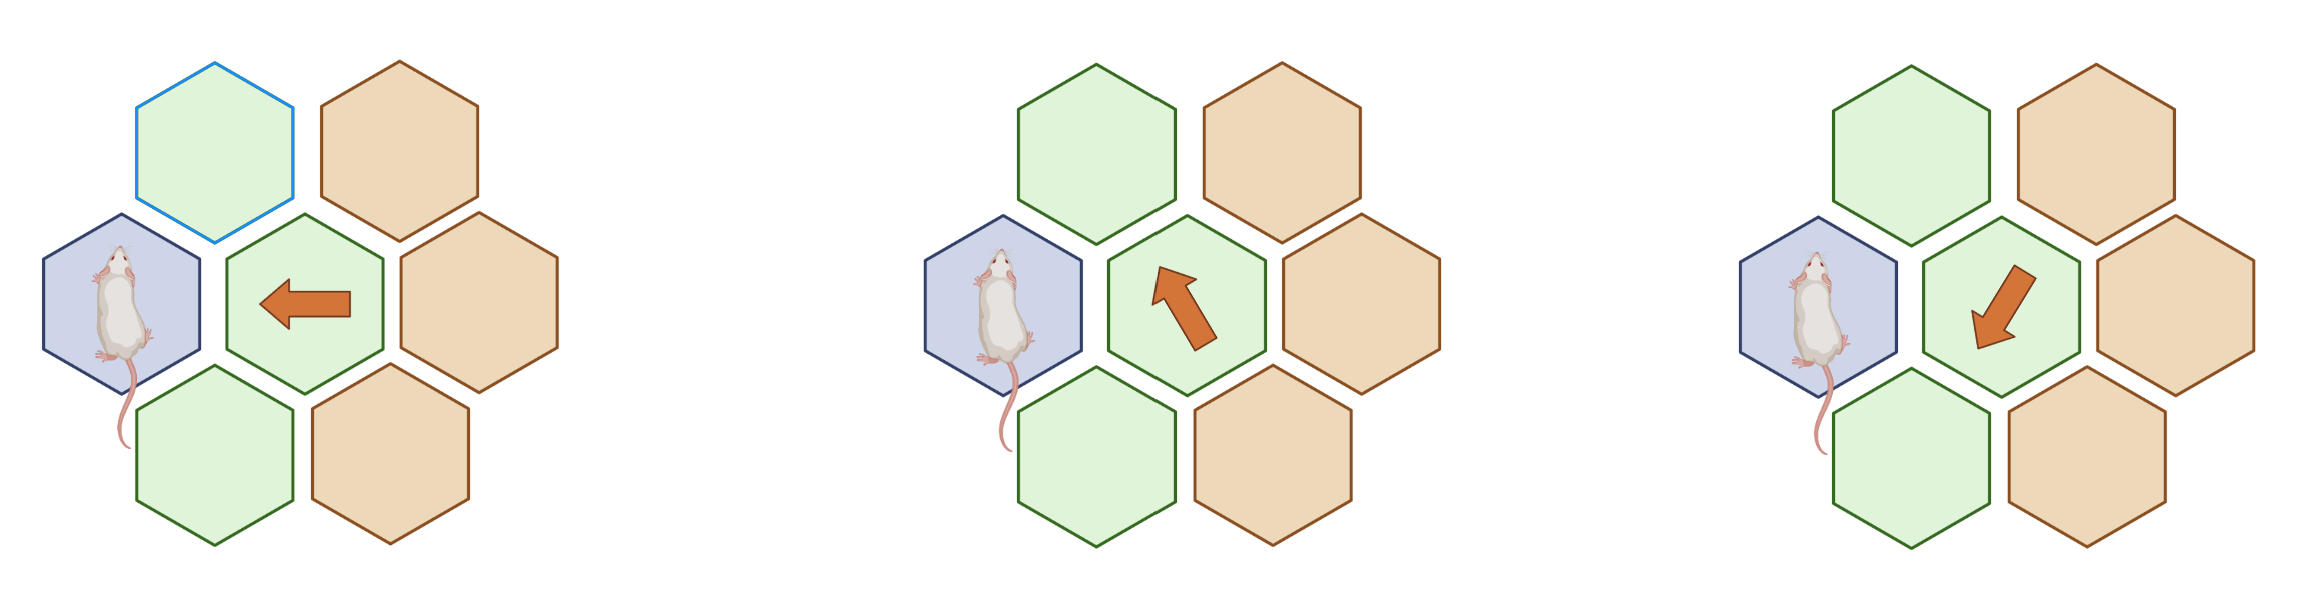
\includegraphics[scale = 0.5]{images/move_to_outer_ring.png}
    \caption{This figure demonstrates that whatever the position of the 'non-animal robot', it must step into the outer ring of the new 'animal robot'. This either means stepping forward once or backwards once, depending on what which was forward is each each of these arrangement. Importantly, note that is always possible for the 'non-non-animal robot' to move the outer ring.}
    \label{fig:nnar_move_to_outer_ring}
\end{figure}

\begin{tcolorbox}
Therefore, in the pre-pathfinding phase of the algorithm:
\begin{enumerate}
    \item NNAR will always move (first) way from the NAR.
    \item NAR will always move (second) into the outer ring of the AR.
\end{enumerate}
\end{tcolorbox}

\subsubsection{Pathfinding Phase}
\label{section:pathfinding}

\paragraph{Justification of \textit{networkx} approach} 

A general path-finding algorithm was implemented, instead of a hard-coded' solution more specific to the task at hand, because a general path-finding algorithm allows a more versatile version of the program handling more combinations of robot positions without the algorithm failing to find a valid path.

To prevent having write source code for a general path finding algorithm, a python library, able to find the shortest path between two points on a network, called \textit{networkx} \cite{networkx} was used instead. This requires the path finding problem presented to be converted into a graph which the library can handle.

The most advanced path-finding algorithm \textif{networkx} supports is the \textit{Dijkstra} path-finding algorithm \cite{dijkstra1959pathfinding}. Though it is not as efficient or versatile as other path-finding algorithms, such as the A*  path-finding algorithm \cite{A*_pathfinding} \cite{lit_review_pathfinding}, for the size and complexity of network that will be generated for the honeycomb maze, the Dijkstra path-finding algorithm will  suffice. Due to the computational time required to find the path being negliable compared with the time taken for the path found to be executed by the robots.

\paragraph{Implementation of \textit{networkx}}
From the hexagonal grid determined by the \textit{Maze} class, a triangular lattice network of the correct size is generated. This encodes all positions (coordinates) that are possible for the robots are able to move to in the room. A triangular lattice is used as this network connects all nodes (not on the boundary of the grid) to six consecutive nodes, which is the same as the number of adjacent movements possible from each point on the grid.


After the whole movement network was generated, a modified version of the movement network was generated: the \textit{temporary movement network (TMN)} with all moves that would cause collision being removed from the network. When a robot wants to move around the network the positions of the 'non-moving' robots were removed from the \textit{TMN} as well as the \textit{inner-ring} positions for these same robots - as these are the positions that would cause collisions if the robot was moved there.
The \textit{TMN} would be returned to the moving robot, where it would find its path from the \textit{path-finding source} to the \textit{path-finding target}.

\begin{figure}[h]
    \centering
    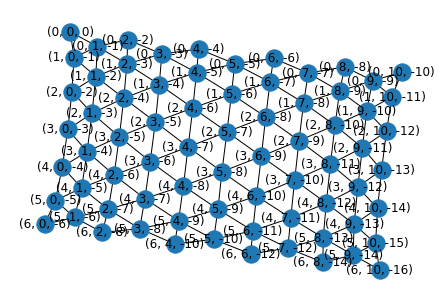
\includegraphics[scale = 0.3]{images/output.png}
    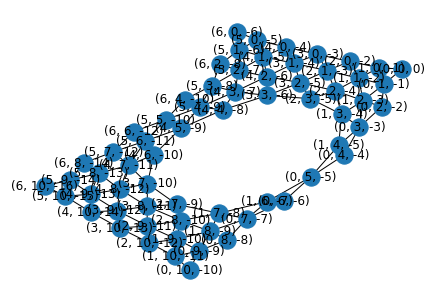
\includegraphics[scale = 0.3]{images/output2.png}
    \caption{This shows an example of the network generated by the \textit{networkx} library (LHS image), based on all the possible moves available in the maze. Once the network has been generated, the positions that are impossible to access by the moving robot are removed from the network (RHS image). From this, the shortest path from the \textit{path-finding source} to the \textit{pathf-inding target} will be found and a list of coordinates that describe the path will be generated and return to the robot. This figure has been generated by the \textit{networkx} package \cite{networkx}.}
    \label{fig:networkx_diagrams}
\end{figure}


\paragraph{Setting Path-finding Targets}
\label{section:pathfinding_targets}

Since the actual source and target of the complete algorithm will always be in the inner ring of the 'non-moving' robots, they are removed from the \textit{TMN}.  As such, they can not be used as the path-finding source and target for the path-finding algorithm. 

Therefore, the source and target used, are corresponding outer ring positions of the actual source and target. They way these are calculated, corresponds to the mapping shown Fig \ref{fig:pathfinding_source_target_mapping} from the (blue) inner relative positions to the (pink) outer relative positions.

This allows the moving robot to get to the correct relative position of its target position, however instead of being in the inner ring, where it aims to be, it is in the outer ring.
% From Fig. \ref{fig:inner_ring}, it can be seen that to get to the inner ring for each relative position, the robot must reach the corresponding relative position on the outer ring and simply move one step towards the animal robot to reach its final position.

% This mapping of every position of the \textit{inner ring} to a position in the \textit{outer ring} has been called \textit{relative position} and can be calculated from the position of any given platform robot. See Table \ref{table:relative_position_truth_table} and Function \ref{function:def_relative_position} for its implementation.

% Based on the \textit{relative position} of the actual goal platform, the path-finding goal is generated by finding the \textit{outer ring} counterpart of the \textit{inner ring} with the same relative position. This is done so that once the robot reaches the outer ring relative position, a standard algorithm can be used to turn the NAR or NNAR to the AR and then step forward (at the same time) to become adjacent to the robot at the same time (see Function \ref{function:move_to_inner_ring)}

\begin{figure}[h]
    \centering
    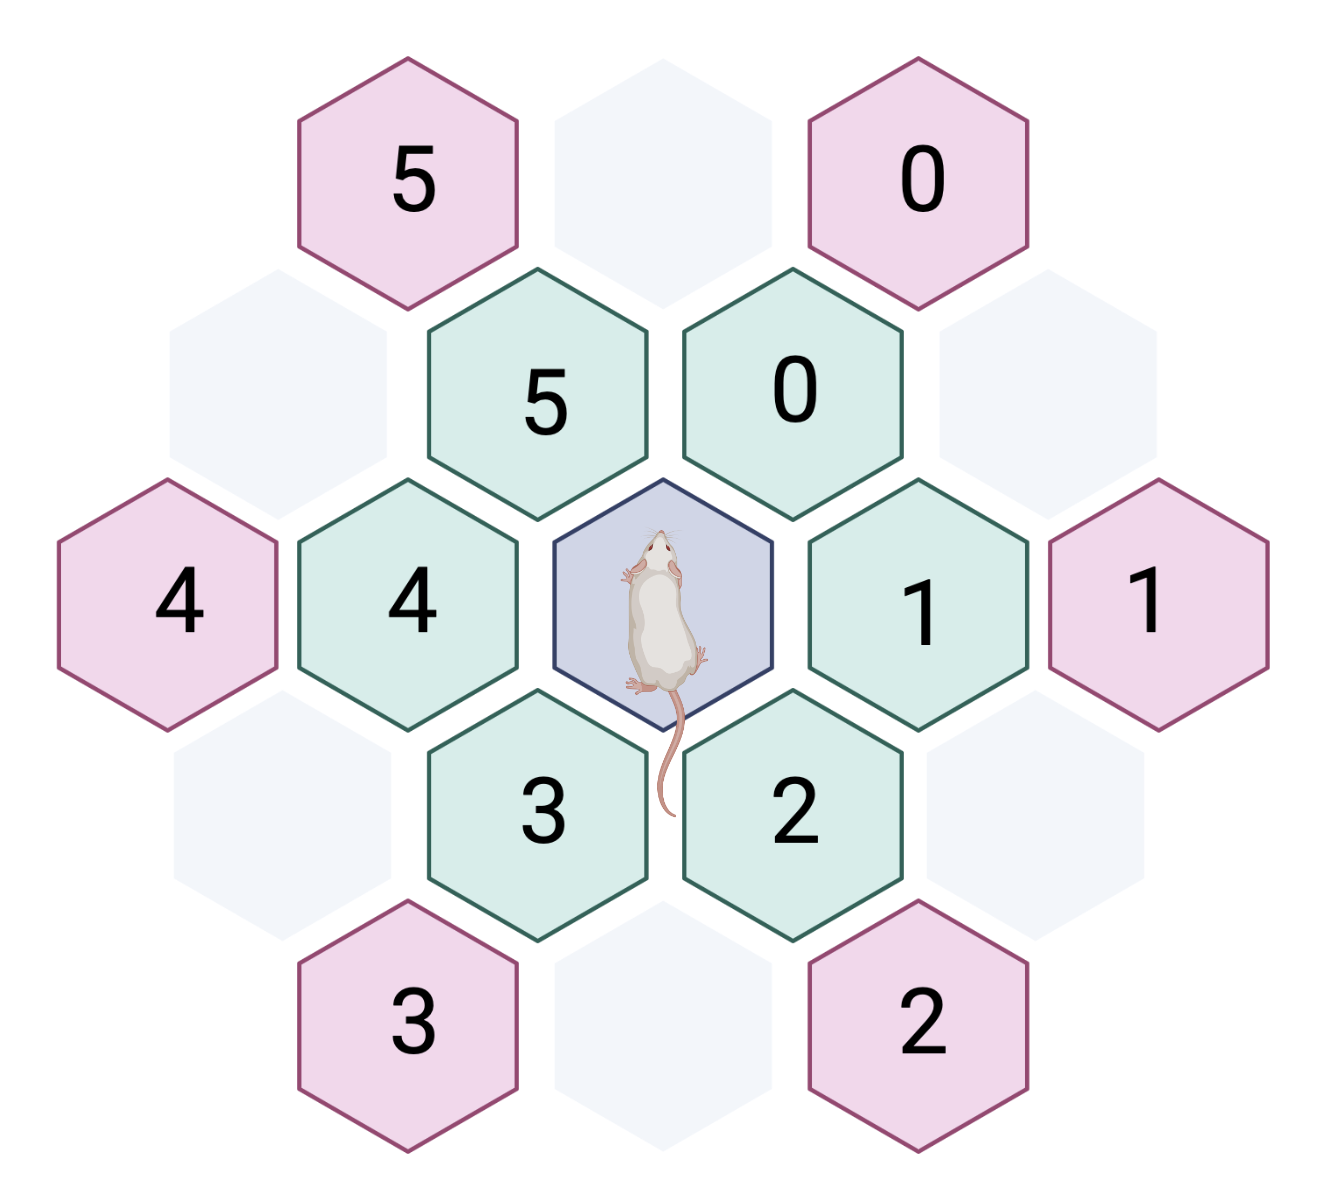
\includegraphics[scale=0.25]{images/pathfinding_source_target.png}
    \caption{This figure shows the mapping from the actual source (or target) of the pathfinding algorithm (in blue) to the 'pathfinding source' or 'pathfinding target'  (in pink). This is because \textit{networkx} will not be able to pathfind from a position in the network that is not present. As such, the pathfinding begins after the 'step back from the NAR' move takes place.}
    \label{fig:pathfinding_source_target_mapping}
\end{figure}

\subsubsection{Post-Path-finding Phase}
\label{section:post_path_finding}

As shown in Fig. \ref{fig:nnar_move_to_outer_ring}, after the animal has made its decision, the NNAR must move to the outer ring to make sure that it does not collide with the NAR when executing its path.

The NNAR, which moves first will wait until, the NAR has moved to its path-finding source. Once both of the moving robot (NAR and NNAR) have reached the end of their pathfinding phase, they will both be in the outer ring of their correct relative position. 
They must both move to from their outer ring position to their equivalent position in the inner ring. This is what occurs in the \textit{Post-Dijsktra Phase} of the algorithm. 

The NNAR will wait for the NAR to be in position. Once this has occurred, both NAR and NNAR will move from their \textit{outer ring} position to their corresponding \textit{inner ring} position, providing a choice for the animal to choose which platform it would like to move to.
This command will be executed at the same time for both robots. This makes sure the animal has the same amount of time to consider each platform, reducing bias to a particular platform.


\subsubsection{Moving to final position}

Once the robots has reached their path-finding target, it will be in the in the correct relative position of the required target, however it will be in the outer ring, not the inner ring (as required). Therefore, a move to the inner ring from the outer ring is all that is required to move to its correct position. (In Fig \ref{fig:pathfinding_source_target_mapping}, they will have to move from the (pink) outer ring to the corresponding position (blue) position in the inner ring.

% From combining the ideas from Figure \ref{fig:inner_ring}, it can be seen that the relative positions is a one to one mapping of the six positions on the inner ring to six positions on the outer ring. This becomes very useful because once a robot on on the outer ring position (where the relative position is defined), it can be used to move the robot from the inner ring to the outer ring in a standard way.

% Once the robot has got to the outer ring of the animal robot, where the relative position is defined, all that the robot has to do is to move from the outer ring to the inner ring whilst staying on the line of the same relative position.

% The non animal robot (or non-non animal robot) simply has to point towards the animal robot. Once it has done this, the animal robot simply has to step once forward. Then it will be consecutive to the animal robot. Once this has occurred the animal can make a decision about which robot platform it would like to move  towards.

Both the \textit{NAR} and \textit{NNAR} will be pointing towards to \textit{AR} when they step forward to get from the outer ring to the inner ring. This means they will \textit{always} be pointing towards the \textit{AR} in their final position. Therefore, the start positions shown in panel A of Fig \ref{fig:control_flow_diagram} are all the valid starting positions that the algorithm must handle.

\\ \\ 

This method of doing the final step in the algorithm means that the platforms can never reach an arrangement where it is hard to deal with their movement. This is because both the non-animal robot and the non-non animal robot will always point towards the animal robot (as is shown in panel A of Fig \ref{fig:control_flow_diagram}) and not be locked into an arrangement which requires a different order of operations that what was described in Section \ref{section:order_of_operations}. 

\pagebreak
\subsection{\textit{Animal} Class}

This class is defines the position of the animal, which must always be on one of the robot platforms. The \textit{animal} class is also used for to model the decision making that the animal made when testing the program.


\subsubsection{Animal class decision making}

Inside this class of the program, the animal robot can interface with \textit{deeplabcut} via simple function which takes the input of which platform the animal has choose to move to.

For testing the program, a simple random decision is made between the two possible choices of platform to move to for testing purposed